%
% HICSS-60 submission — Dependable Technical and Socio-technical Systems Engineering minitrack
% Initial manuscript (NO author names — double-blind). Max 10 pages incl. references.
% Requires hicss-packages.tex (official HICSS template) + references.bib in same folder.
%
% ============================================================
%  DATA VERSION NOTES (update when more seeds arrive)
%  u20 primary:  N=5 seeds, PureDRL fail=3/5=60%, Proposed=0/5=0%
%  Statistical test: binomial p=0.010 on u20 failure counts
% ============================================================
\documentclass[10pt]{article}
%
% hicss-packages.tex
% HICSS-60 compatible package and layout settings
% Based on HICSS official formatting guidelines (10pt, Times, two-column, 1-inch margins)
%

% --- Page geometry ---
\usepackage[letterpaper,
            top=1in, bottom=1in,
            left=1in, right=1in]{geometry}

% --- Two-column layout ---
\usepackage{multicol}
\twocolumn
\setlength{\columnsep}{0.33in}

% --- Fonts ---
\usepackage{times}
\usepackage[T1]{fontenc}
\usepackage[utf8]{inputenc}

% --- Math ---
\usepackage{amsmath,amssymb}

% --- Graphics ---
\usepackage{graphicx}
\usepackage[table]{xcolor}   % required for \cellcolor in tables

% --- Tables ---
\usepackage{booktabs}
\usepackage{multirow}
\usepackage{array}
\usepackage{tabularx}

% --- Prevent text overflowing column ---
\emergencystretch=2em

% --- Bibliography (biblatex + bibtex) ---
\usepackage[backend=bibtex,
            style=authoryear,
            sorting=nyt,
            maxbibnames=6,
            minbibnames=3,
            uniquename=false,
            uniquelist=false]{biblatex}

% --- Hyperlinks (load last) ---
\usepackage[colorlinks=true,
            linkcolor=black,
            citecolor=black,
            urlcolor=black]{hyperref}

% --- Section title formatting ---
\usepackage{titlesec}
\titleformat{\section}{\normalfont\large\bfseries}{\thesection.}{0.5em}{}
\titleformat{\subsection}{\normalfont\normalsize\bfseries}{\thesubsection}{0.5em}{}
\titleformat{\subsubsection}{\normalfont\normalsize\itshape}{\thesubsubsection}{0.5em}{}

% --- Caption formatting ---
\usepackage{caption}
\captionsetup{font=small, labelfont=bf}

% --- Spacing ---
\usepackage{setspace}
\setlength{\parskip}{0pt}
\setlength{\parindent}{1em}

% --- Figure/table placement ---
\usepackage{float}

% --- Checkmark / cross symbols ---
\usepackage{pifont}
\newcommand{\cmark}{\ding{51}}   % heavy checkmark
\newcommand{\xmark}{\ding{55}}   % heavy x

% --- Misc ---
% \usepackage{microtype}  % disabled: causes compile timeout on Overleaf free plan
\usepackage{enumitem}
\setlist[itemize]{topsep=2pt, itemsep=1pt}

\newcommand{\sansserifformat}[1]{\fontfamily{cmss}{ #1}}%

\addbibresource{references.bib}

\title{LLM-Governed Hierarchical DRL for Dependable Scheduling
in Nondeterministic Digital Twins}

\date{}

\begin{document}
\maketitle

% ============================ ABSTRACT (<=150 words) ============================
\begin{abstract}
\textit{%
Deep Reinforcement Learning (DRL) is increasingly applied to manufacturing
scheduling, but its learned policies can be unreliable: under the inherent
nondeterminism of a high-fidelity digital twin, identically configured training
runs sometimes converge to good policies and sometimes fail catastrophically.
We study urgent-lot scheduling in a semiconductor-manufacturing digital twin and
show that, when urgent lots are sufficiently frequent to create scheduling
conflicts, DRL fails catastrophically in 60\% of independent runs.
We propose a three-layer Hierarchical RL framework in which a
locally hosted Large Language Model (LLM) acts as an episodic governance layer
generating safety rules that constrain the DRL agent.
Across 5 independent seeds, Pure DRL failed in 60\% of runs while the
LLM-governed agent failed in 0\%, reducing cycle-time variance by 73\%
with no loss of production attainment.
We frame LLM governance as a fault-tolerance mechanism that improves
the dependability of learned components in socio-technical manufacturing
systems.%
}
\end{abstract}

\subsubsection*{Keywords:}
Dependable AI; Deep Reinforcement Learning; Large Language Models; Digital Twin;
Manufacturing Scheduling

% ============================ 1. INTRODUCTION ============================
\section{Introduction}

Semiconductor-manufacturing lines are stochastic, non-stationary scheduling
environments. A single dispatching decision can reshape the work-in-process
(WIP) distribution and influence cycle time tens of minutes or even hours later,
so a scheduler's action at time $t$ carries long-horizon consequences that are
hard to attribute and harder to optimize with fixed heuristics
\parencite{moyne2017,hu2019}. To cope with this complexity, recent research couples a
\emph{digital twin} (a high-fidelity discrete-event simulation of the line) with
Deep Reinforcement Learning (DRL), learning a dispatching policy directly from
the simulated environment \parencite{waschneck2018,lee2025}.
Figure~\ref{fig:drl_framework} illustrates this baseline coupling: a
manufacturing digital twin supplies shop-floor state and receives dispatching
actions, while a Rainbow DQN agent learns via experience replay through its
Q-Network and Target-Network pair.

\begin{figure}[h]
  \centering
  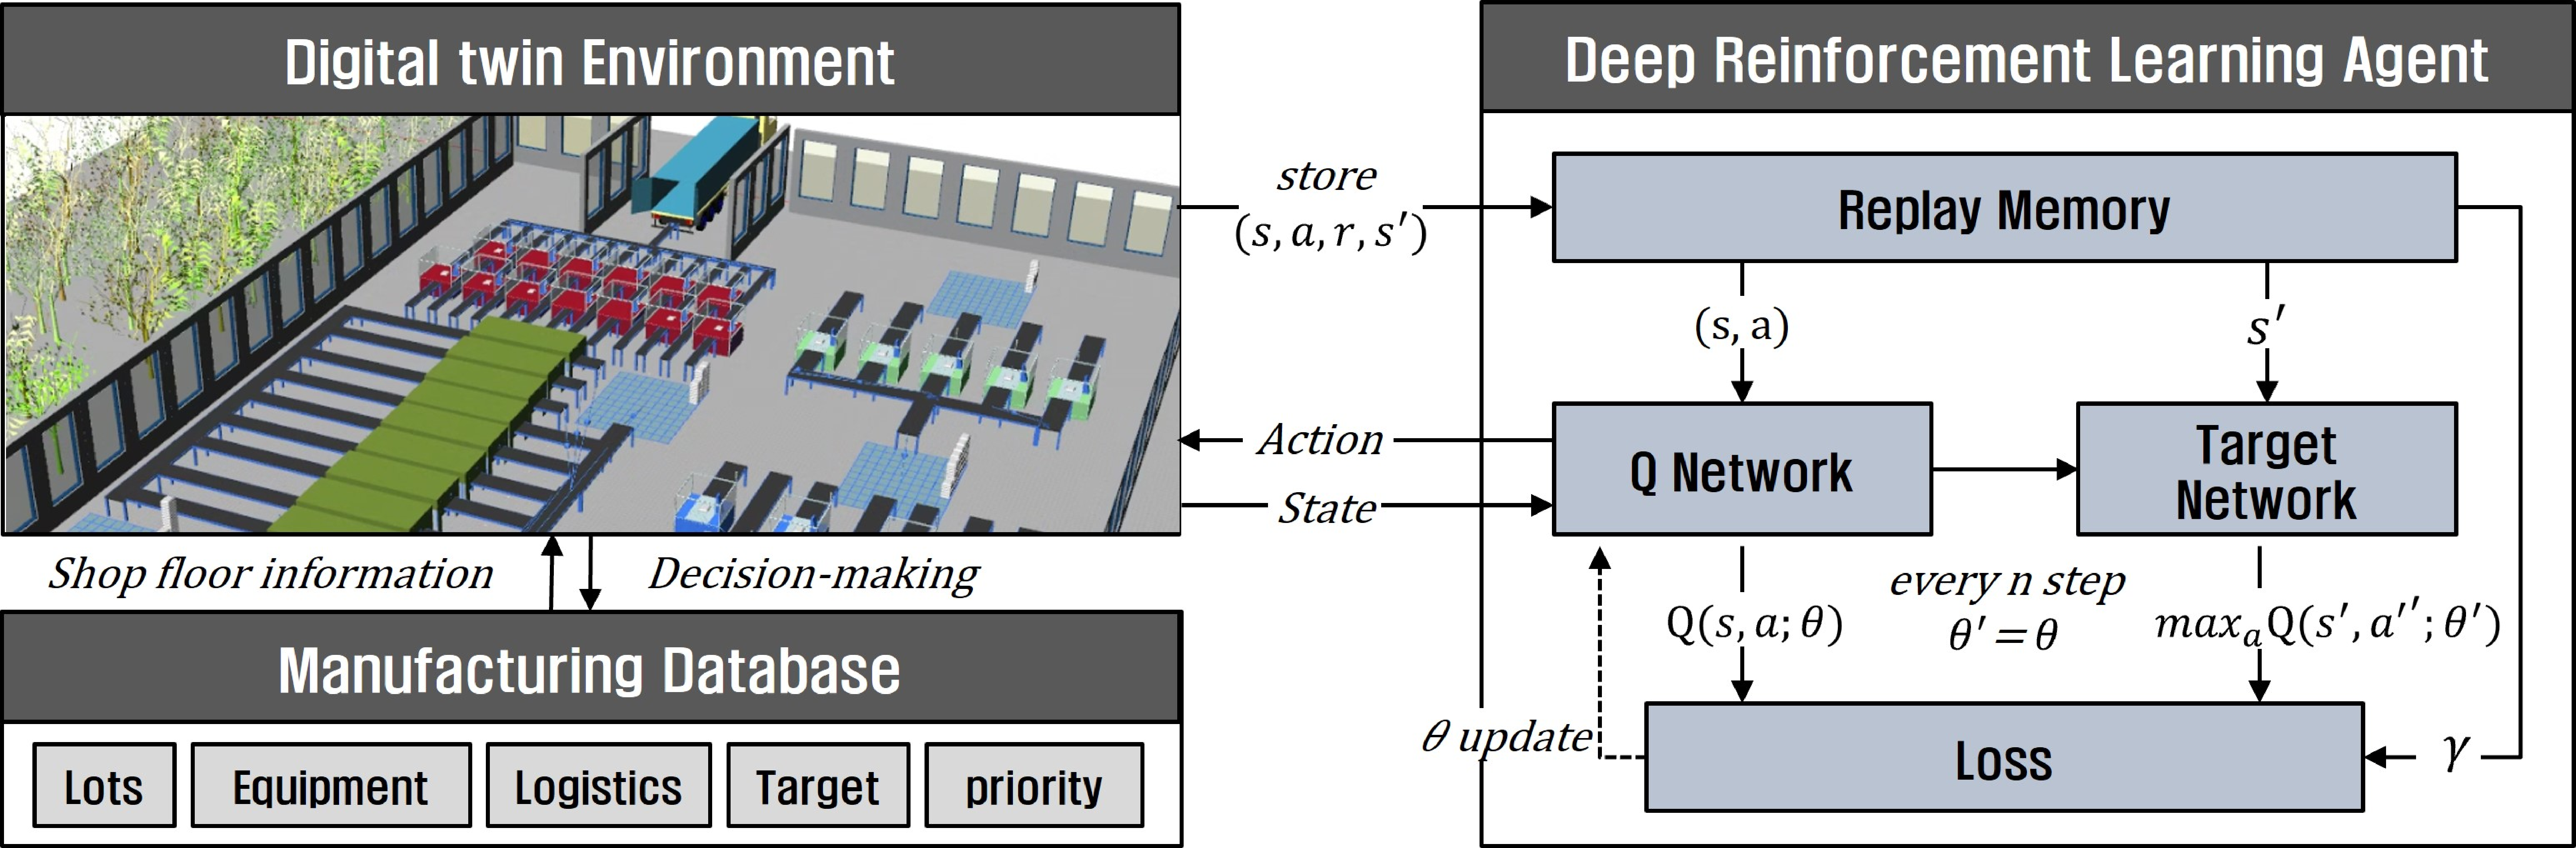
\includegraphics[width=0.98\linewidth]{DRL_Framework}
  \caption{Baseline DRL scheduling framework. The digital twin acts as the
    training environment; the agent observes shop-floor state $s$, selects a
    dispatching action $a$, and updates its Q-Network weights $\theta$ via
    the Bellman loss $\mathcal{L}(\theta)=\bigl(Q(s,a;\theta)
    -[r+\gamma\max_{a'}Q(s',a'';\theta')]\bigr)^{2}$,
    with the Target Network $\theta'$ synchronized every $n$ steps.}
  \label{fig:drl_framework}
\end{figure}

Despite encouraging average-case results, deploying DRL in cost- and
yield-critical manufacturing surfaces a \emph{dependability} concern that the
literature rarely quantifies: the learned policy is not reliable from run to run.
In this paper we demonstrate that, owing to the internal nondeterminism of the
digital twin, \emph{identically configured and seeded} DRL training runs can converge to a
high-quality policy in one run and fail catastrophically in another. This
fragility is most acute when urgent-lot conflicts arise: a small cohort of
high-priority lots must traverse the line as quickly as possible, but when they
are numerous enough to create genuine contention at bottleneck stages, the reward
signal becomes noisy and the agent's convergence becomes a matter of chance.

This run-to-run unreliability falls squarely within the purview of
\emph{dependability engineering} \parencite{avizienis2004}: the scheduler exhibits an
intermittent fault that occasionally produces a failed schedule under nominally
identical conditions. The question we pose is not ``how do we make DRL faster on
average?'' but rather ``how do we make an \emph{unreliable} DRL scheduler
\emph{dependable}?''

We answer this question with a three-layer Hierarchical Reinforcement Learning
(HRL) framework in which a Large Language Model (LLM) provides
\emph{strategic governance} over a tactical DRL agent. After each training
episode, the LLM inspects aggregated Key Performance Indicators (KPIs) and emits
a small set of safety rules; these rules are compiled into per-step action masks
that constrain the DRL agent. Crucially, the LLM is hosted \emph{locally}, with no external API call. We
show that this lightweight, low-frequency governance does not merely shift the
mean: it removes the catastrophic-failure tail, converting an unreliable agent
into a dependable one.

Our contributions are threefold.
\begin{itemize}
\setlength\itemsep{0em}
\item \textbf{Empirical characterization of DRL unreliability under digital-twin
nondeterminism.} We show that the same configuration fails in 60\% of
independent runs at the critical sparsity regime, and that this variance
appears to originate from simulator-level nondeterminism rather than controllable random seeds
(Sections~\ref{sec:setup} and~\ref{sec:results}).
\item \textbf{LLM governance as a fault-tolerance layer.} We demonstrate that
episodic LLM-generated rules reduce the catastrophic-failure rate from 60\%
to 0\% and cut cycle-time variance by 73\% without sacrificing production
targets, and we explain the mechanism: sparse but well-timed interventions during
training teach the agent a behavior it otherwise acquires only unreliably.
\item \textbf{Deployment lessons for local-LLM rule generation.} We report
systematic rule-generation error patterns of a 7B local model and the prompt-
and code-level guardrails that made deployment safe, an engineering ``means''
for dependable LLM-in-the-loop control.
\end{itemize}


% ============================ 2. RELATED WORK ============================
\section{Related work}
\label{sec:related}

Our work sits at the intersection of three threads: DRL for manufacturing
scheduling, sparse rewards and exploration, and LLMs guiding reinforcement
learning. We review each and position our contribution.

\subsection{DRL and digital twins for scheduling}
Reinforcement learning has been applied to semiconductor dispatching and scheduling
as an alternative to static rule-based policies, which struggle with the
long-horizon, re-entrant nature of these lines \parencite{waschneck2018,hu2019}.
A common pattern pairs a discrete-event digital twin with a value-based agent
that selects among dispatching rules at each decision point \parencite{lee2025}. The
Rainbow DQN architecture \parencite{hessel2018}, which we adopt for the tactical
layer, combines several stabilizing techniques (double Q-learning, dueling
networks, prioritized replay, noisy exploration, and multi-step returns) and is a
strong default for discrete-action control. However, this literature
overwhelmingly reports \emph{mean} performance over a small number of runs and
seldom analyzes \emph{reliability} (the distribution of outcomes across
independent trainings), which is exactly the property that matters when a single
bad schedule incurs large, yield-critical losses. Our study foregrounds this
distributional view. The suitability of DRL for this dispatching setting is
taken as an established premise: \textcite{lee2025} demonstrated that DRL
outperforms static heuristics in the same nondeterministic manufacturing scheduling
environment; the present work accepts that baseline and asks how to make
DRL-based scheduling \emph{dependable} rather than merely effective on average.

\subsection{Sparse rewards and exploration}
A well-known obstacle for DRL is the sparse-reward problem: when the events that
should be rewarded are rare, the agent receives little signal and may settle into
a local optimum that ignores them \parencite{pathak2017}. Table~\ref{tab:sparse}
compares the three principal responses to this problem in the context of
manufacturing dispatch.

\begin{table}[thb]
\centering
\caption{Responses to the sparse-reward problem in manufacturing dispatch.}
\label{tab:sparse}
\setlength{\tabcolsep}{4pt}
\footnotesize
\begin{tabularx}{\columnwidth}{@{}p{2.1cm}XX@{}}
\hline
\textbf{Approach} & \textbf{Mechanism} & \textbf{Key limitation} \\ \hline
Reward shaping (\citeyear{ng1999})
                   & Augments or rescales the reward signal to make rare events more salient.
                   & Creates a non-stationary learning target;
                     distorts the signal during normal operation. \\[2pt]
Intrinsic motivation (\citeyear{pathak2017})
                   & Adds an exploration bonus toward under-visited states.
                   & Does not guarantee \emph{which} rare behaviors are learned;
                     does not bound outcome variance. \\[2pt]
\textbf{Action-space constraint (ours)}
                   & Prunes unsafe actions via an external governor,
                     leaving the reward function intact.
                   & Requires a rule source that can identify which actions
                     to constrain and update them as conditions change. \\ \hline
\end{tabularx}
\normalsize
\end{table}

In manufacturing, the rare-but-critical event (an urgent lot, a quality-time
violation) is precisely where a guarantee is most valuable. Reward shaping
addresses frequency but introduces a non-stationary training target: a weight
large enough to dominate at conflict time distorts the signal during the far
more frequent non-conflict periods, increasing training variance. We instead
constrain the action space through an external governor, steering the agent
toward the desired behavior without altering its reward function.
The natural follow-on question is: which type of external governor is best
suited to this task?

\subsection{Why LLM governance: motivating the design choice}
\label{sec:alternatives}

The sparse-reward problem established in the previous section calls for an
external mechanism that can steer the DRL agent toward urgent-lot handling
without distorting the reward signal.
Table~\ref{tab:alternatives} surveys the principal alternatives and identifies
why each falls short in our setting.

\begin{table}[thb]
\centering
\caption{Alternative approaches to urgent-lot scheduling and DRL reliability
in nondeterministic manufacturing environments.}
\label{tab:alternatives}
\setlength{\tabcolsep}{4pt}
\footnotesize
\begin{tabularx}{\columnwidth}{@{}p{2.3cm}X@{}}
\hline
\textbf{Approach} & \textbf{Key limitation in our setting} \\ \hline
Rule-based dispatch (\citeyear{waschneck2018})
  & Requires domain experts to enumerate all exception conditions; brittle
    when novel conflict patterns arise outside the rule vocabulary. \\[2pt]
Constraint programming (\citeyear{baptiste2001})
  & Exact solvers are too slow for real-time dispatch; stochastic
    arrivals and processing times degrade solution quality. \\[2pt]
MORL (\citeyear{hayes2022})
  & Objective weights are fixed at design time; cannot adapt prioritization
    to dynamic conflict conditions without reward redesign and retraining. \\[2pt]
\textbf{LLM-HRL (ours)}
  & Leverages natural-language domain knowledge for zero-shot contextual
    prioritization; no retraining required when conflict conditions change. \\ \hline
\end{tabularx}
\normalsize
\end{table}

Although the reward function (Eq.~\ref{eq:reward}) has a superficially
multi-objective character, the mechanism differs fundamentally from MORL: rather
than fixing scalar weights at design time, the L2 governor \emph{dynamically
constrains the action space} only when KPIs signal an active urgent-lot conflict,
leaving the reward signal undistorted during normal operation.
Having established that LLM-based governance is the appropriate design choice,
we now review how existing LLM-guided RL approaches compare with our framework.

\subsection{LLMs guiding reinforcement learning}
Large language models have recently been used to inject high-level knowledge into
RL. Approaches include decomposing long-horizon goals into sub-goals to guide
early exploration \parencite{du2023}, grounding LLMs in interactive environments via
online RL \parencite{carta2023}, and translating natural-language or code instructions
into executable policies \parencite{liang2023}. A complementary line encodes safety as
formal constraints, e.g.\ translating instructions into temporal logic to prune
unsafe actions \parencite{hasanbeig2020}. Our framework differs in two ways. First,
governance is \emph{continuous and KPI-driven}: the LLM re-evaluates the line's
state every episode and revises its rules, rather than providing static initial
guidance. Second, governance is \emph{decoupled by frequency}: the LLM operates
at the episode timescale (seconds of inference are acceptable), while a
lightweight safety agent enforces the resulting rules at the millisecond
dispatch timescale, an arrangement aligned with hierarchical RL, in which a
high-level manager sets goals for a low-level worker \parencite{vezhnevets2017}.

Table~\ref{tab:related} summarises how our framework compares to the most closely
related lines of work along four dimensions that matter for industrial deployment.

\begin{table}[thb]
\centering
\caption{Comparison of LLM-guided RL approaches on four deployment-relevant
dimensions. ``Freq.'' = how often LLM guidance is applied;
``Safe'' = explicit action constraints;
``Interp.'' = human-readable rationale; ``Dep.'' = validated by
failure-rate reduction.}
\label{tab:related}
\setlength{\tabcolsep}{4pt}
\footnotesize
\begin{tabularx}{\columnwidth}{@{}Xccccc@{}}
\hline
\textbf{Approach} & \textbf{Freq.} & \textbf{Safe} & \textbf{Interp.} & \textbf{Dep.} \\
\hline
\textcite{du2023}        & One-shot  & \xmark  & \xmark  & \xmark \\
\textcite{carta2023}     & Per-step  & \xmark  & \xmark  & \xmark \\
\textcite{liang2023}     & One-shot  & Part.   & Part.   & \xmark \\
\textcite{hasanbeig2020} & Static    & \cmark  & \xmark  & \xmark \\
\textbf{Ours}            & \textbf{Per-ep.} & \textbf{\cmark} & \textbf{\cmark} & \textbf{\cmark} \\
\hline
\end{tabularx}
\normalsize
\end{table}

The key differentiators are the \emph{continuous, KPI-driven} revision cycle
(as opposed to one-shot or static guidance), the explicit \emph{action-space
constraints} that enforce safety at every dispatch step, and the explicit
validation against a \emph{dependability} criterion (failure-rate reduction).


% ============================ 3. SYSTEM ARCHITECTURE ============================
\section{Three-layer governance architecture}
\label{sec:arch}

\begin{figure}[thb]
    \centering
    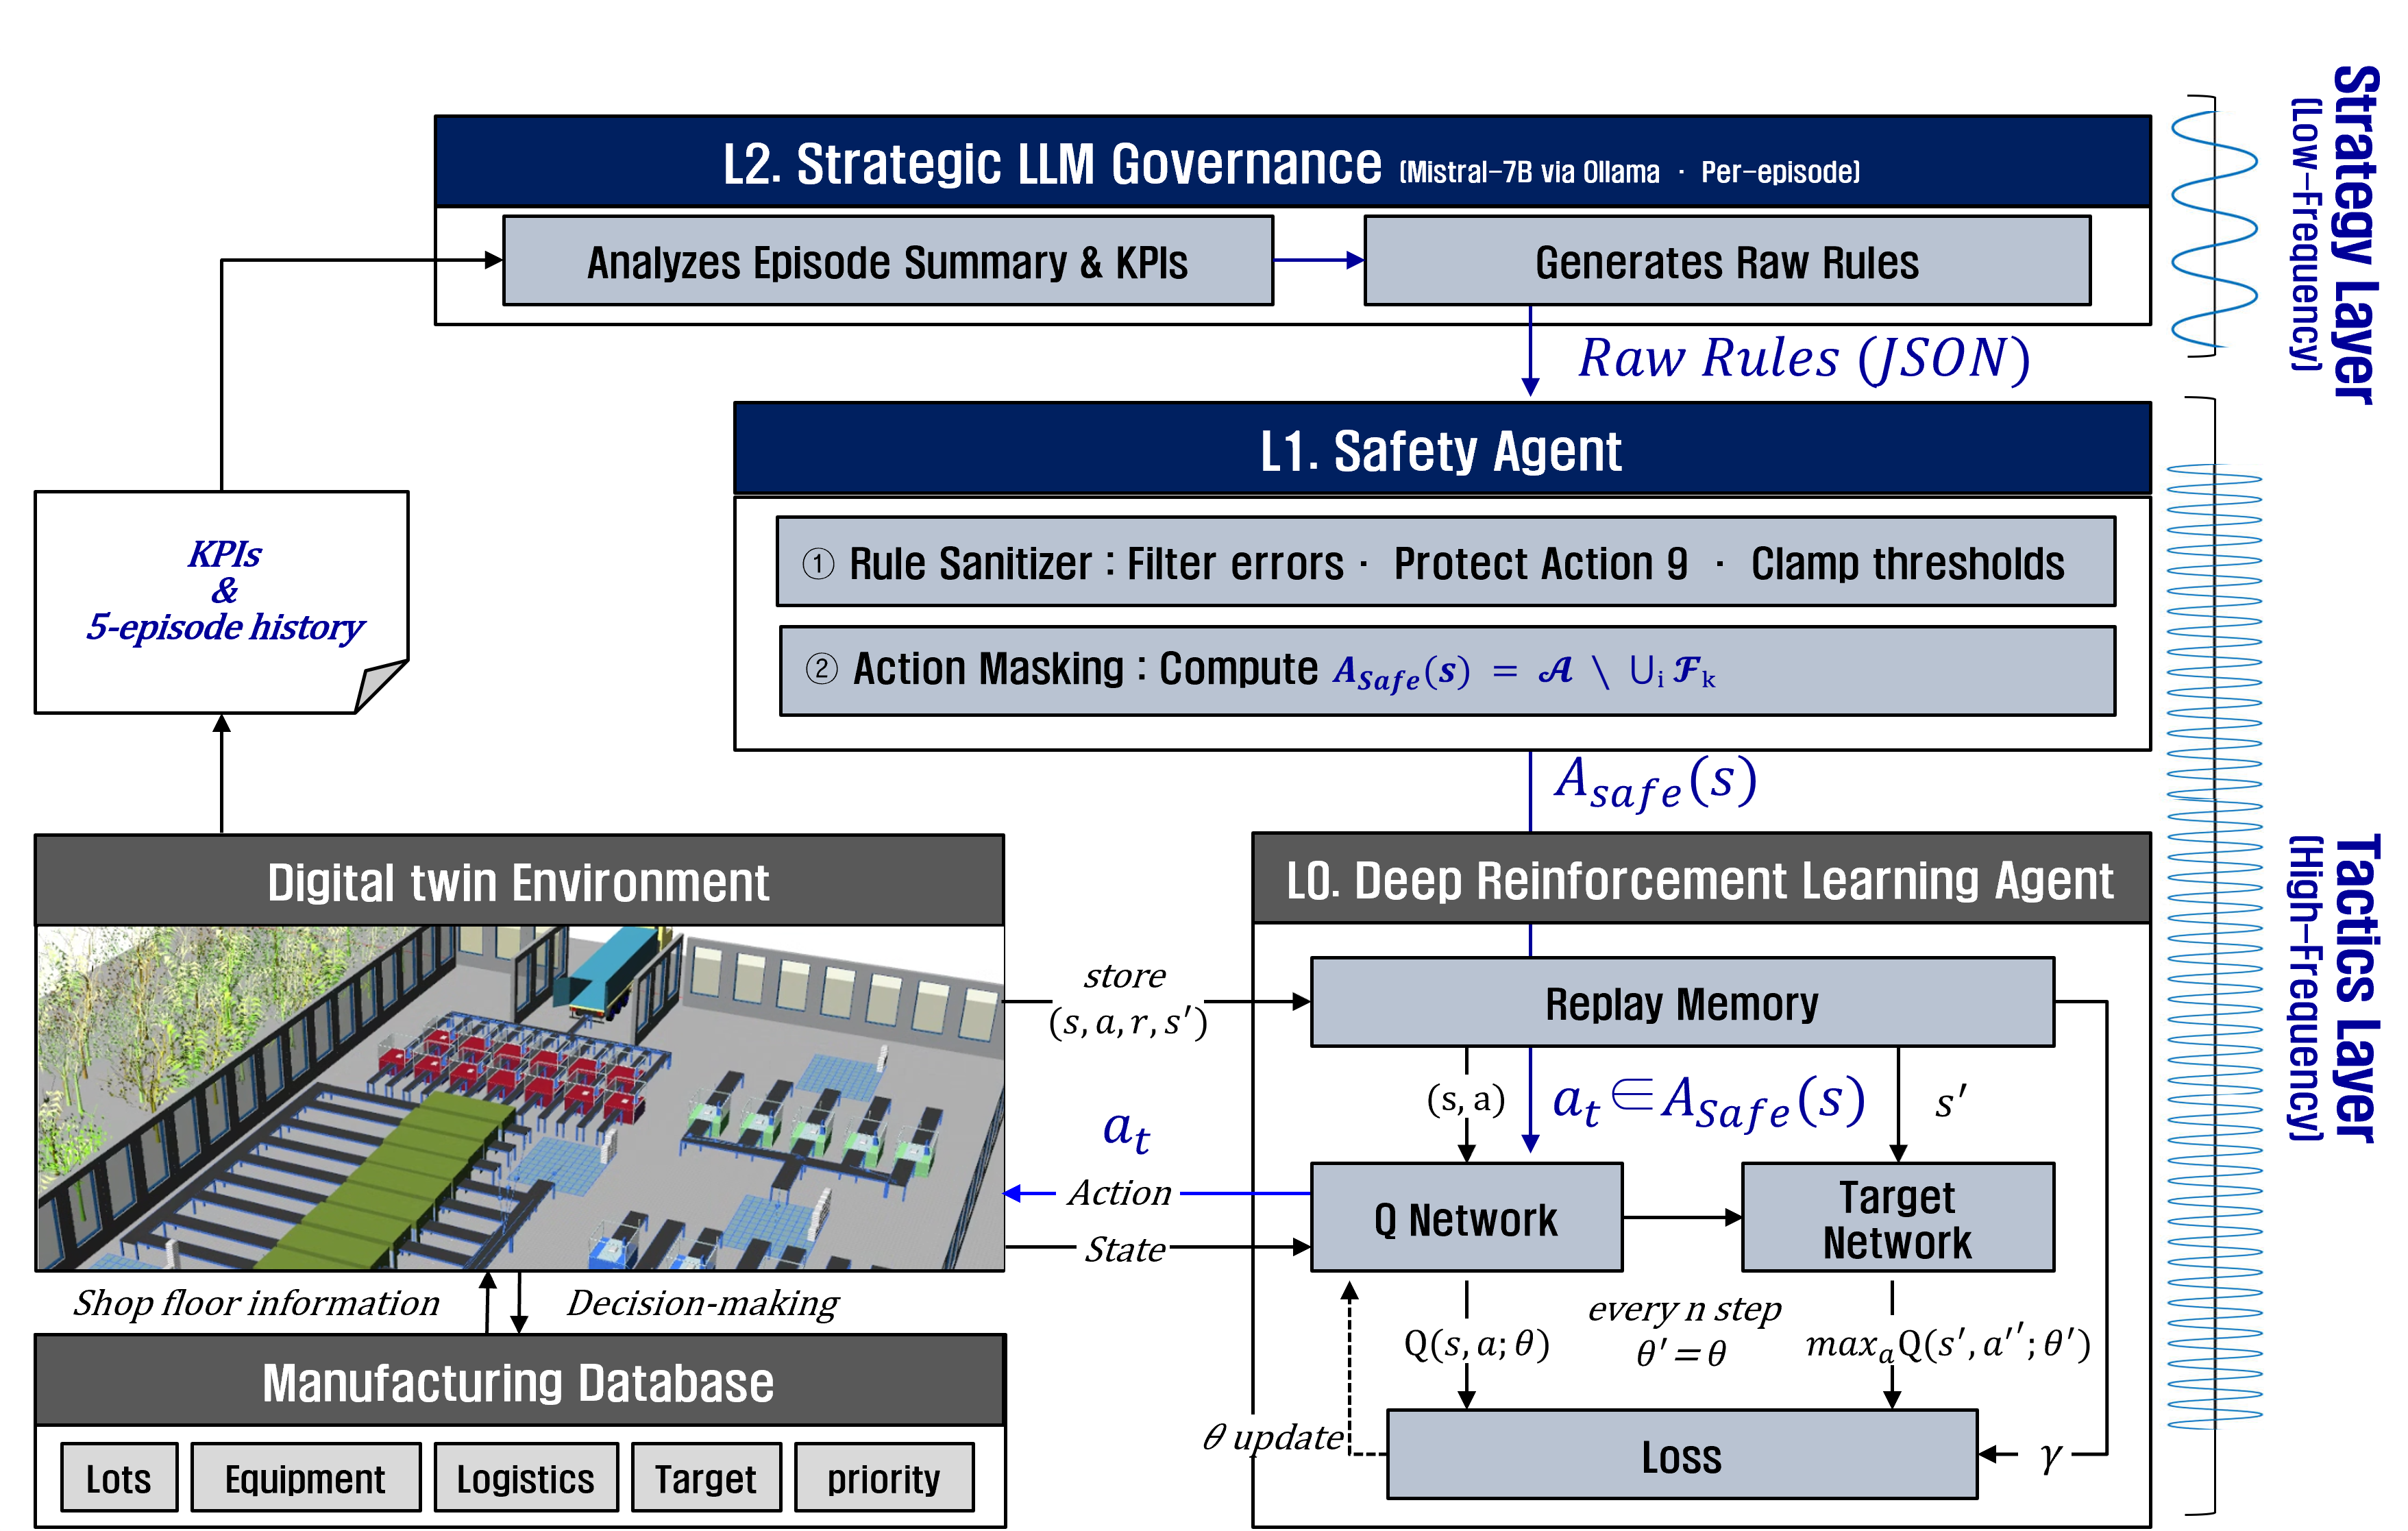
\includegraphics[width=0.98\linewidth]{fig2_architecture_improved}
    \caption{Three-layer governance architecture. L2 (Mistral-7B via Ollama)
    generates episodic safety rules from KPIs; L1 (Safety Agent) validates them
    via a built-in sanitizer and enforces per-step action masks
    (Eq.~\ref{eq:mask}); L0 (Rainbow DQN) selects the highest-value permitted
    action (Eq.~\ref{eq:constrained}). A hard-constraint floor prevents
    governance from sacrificing production attainment.}
    \label{fig:arch}
\end{figure}

Figure~\ref{fig:arch} summarizes the framework, which separates \emph{strategy}
from \emph{tactics} across three layers operating at different time-scales.
Rather than treating the rule sanitizer as a separate architectural layer, it is
embedded within L1 as a pre-processing step: rules arriving from L2 pass through
the sanitizer before being loaded into the enforcement logic.  This keeps the
architecture genuinely three-layer and avoids the overhead of additional
inter-layer communication.

\subsection{L2 -- Strategic governance (local LLM)}
The top layer is a locally hosted LLM that performs episodic governance---the
entry point of the governance chain. After each training episode, it receives the
episode's aggregated KPIs (urgent-lot count and production shortage percentage)
and a five-episode rolling history, and is prompted to
(i) analyze the performance trend, (ii) diagnose the dominant bottleneck, and
(iii) emit zero or more safety rules, each specified as a tuple of (metric,
comparison operator, threshold, forbidden actions). The LLM reasons in natural
language and returns a structured (JSON) response, providing an explicit,
human-readable rationale for every rule it generates, an interpretability
property absent from end-to-end DRL.

Each episode simulates one full day of factory operation (86,400 s), during which
hundreds of event-driven dispatch decisions occur. Because LLM inference takes on
the order of seconds while each dispatch decision occurs in milliseconds, placing
the LLM in the per-step control loop would create an untenable latency bottleneck.
Our \emph{frequency-decoupled} design resolves this: the LLM acts \emph{once per
episode} (one inference call per day of simulated operation), and the resulting
rules are enforced by the lightweight L1 agent at every dispatch step within that
episode. This separation of strategic reasoning from tactical execution is the
defining feature of the hierarchical design.

\subsection{L1 -- Safety enforcement (with built-in sanitizer)}
The middle layer is a lightweight Safety Agent that receives the rule set
$\mathcal{R} = \{r_1, \ldots, r_K\}$ from L2 and enforces it at every dispatch
step. Before enforcement begins, a \emph{built-in rule sanitizer} validates each
incoming rule, discarding logically inverted predicates, protecting the urgent-lot action from
suppression, and clamping thresholds to the per-step evaluation scale.

Each validated rule $r_k$ is a tuple
$(m_k,\, \odot_k,\, \theta_k,\, \mathcal{F}_k)$, where $m_k$ is a KPI metric,
$\odot_k \in \{>, \geq, <, \leq\}$ is a comparison operator, $\theta_k$ is a
threshold, and $\mathcal{F}_k \subseteq \mathcal{A}$ is the set of forbidden
actions when the rule fires.  At each dispatch step, the \emph{safe action set} is
\begin{equation}
  A_{\text{safe}}(s) \;=\; \mathcal{A} \;\setminus\;
  \bigcup_{k:\; m_k(s)\,\odot_k\,\theta_k} \mathcal{F}_k,
  \label{eq:mask}
\end{equation}
and L0 selects
\begin{equation}
  a^* \;=\; \arg\max_{a \,\in\, A_{\text{safe}}(s)} Q(s, a;\,\theta).
  \label{eq:constrained}
\end{equation}
If $A_{\text{safe}}(s) = \emptyset$ (conflicting rules forbid all actions),
a fallback reverts to the unconstrained greedy action, preventing deadlock.
The Safety Agent adds negligible latency and is fully deterministic and
auditable, important properties for a safety component in a socio-technical
deployment.

\subsection{L0 -- Tactical agent (Rainbow DQN)}
The lowest layer is a Rainbow DQN agent \parencite{hessel2018} that operates within
the safe action set defined by L1. It observes a 21-dimensional state vector
$s \in \mathcal{S}$ and selects one of ten dispatching actions at every decision
step. The state concatenates: normalized simulation time (1), process-stage buffer
occupancy per device family (4), production shortage per device (4), in-process
lead-time risk statistics (8), and the count of urgent lots currently waiting at
the critical process stage (4). The ten actions are structured as two categories.
The first category comprises \textbf{nine production-dispatching actions}, encoding combinations of three lot-sorting criteria (by production-quantity deficit, by elapsed wait time, or by remaining deadline proximity) and three equipment-allocation parameters — yielding nine distinct throughput and TMR optimization policies.
The second category is a single \textbf{urgent-lot action} that overrides normal queue order entirely by assigning the highest dispatch priority to all urgent lots; it is the sole mechanism able to advance urgent lots ahead of ordinary scheduling.
This design reflects a deliberate trade-off: the agent must choose, at each dispatch step, whether to optimize production throughput or to serve urgent-lot demand given the current shop-floor state.
The reward function decomposes as
\begin{equation}
  R(s,a) \;=\; R_{\text{prod}}(s,a) \;+\; R_{\text{urgent}}(s,a) \;+\; R_{\text{penalty}}(s,a),
  \label{eq:reward}
\end{equation}
where $R_{\text{prod}}$ captures production attainment, $R_{\text{urgent}}$
rewards reductions in urgent-lot cycle time, and $R_{\text{penalty}}$ imposes
per-step penalties for priority violations. Because urgent lots represent at most
7.7\% of all lots, $R_{\text{urgent}}$ is intermittent and contributes only a
small fraction of the total return, creating the sparse-signal condition studied
in Section~\ref{sec:results}.

\subsection{Hard constraint and production floor}
A \emph{hard constraint} within L1 clears all active rules whenever production
attainment falls below an 85\% floor, ensuring that governance never trades away
the primary production objective in pursuit of urgent-lot performance.
Together with the built-in sanitizer (Section~\ref{sec:lessons}), this guardrail
is the ``fault-removal'' mean that makes an imperfect language model safe to
deploy in the control loop.

% ============================ 4. EXPERIMENTAL SETUP ============================
\section{Experimental environment and setup}
\label{sec:setup}

\subsection{Digital twin and local LLM}
We use a Siemens Tecnomatix Plant Simulation model of a semiconductor line with six
sequential processes (A--F) and heterogeneous equipment at the critical stage.
The model was constructed from actual semiconductor factory data---including
measured lot-arrival distributions, equipment processing times, and routing
constraints---and validated against observed throughput and cycle-time statistics
from the source facility, reproducing lot arrivals, routing, processing, and
buffering over a one-day simulation horizon~\parencite{siemens2023tecnomatix}.

Owing to a research-environment security policy that prohibits sending
production data to external services, no commercial LLM API may be used;
this constraint also reflects typical data-governance requirements in real
semiconductor fabs. We therefore deploy Mistral-7B~\parencite{jiang2023} locally through the Ollama
runtime as the L2 governor, selected for its sufficient instruction-following
capability for structured JSON rule generation and its ability to fit within
consumer GPU memory while keeping per-episode inference latency under 5\,s.
The governance framework is model-agnostic; upgrading to a larger
instruction-tuned model is expected to reduce the observed 14.5\% rule-error
rate without architectural changes.

\subsection{Urgent-lot scenario}
\label{sec:urgentscenario}
A small number of urgent lots (identifiers beginning with ``U'') are injected at
the line entrance and must reach completion as quickly as possible.
Urgent lots in semiconductor fabs arise from multiple operational sources---
evaluation lots, customer samples, critical items, and expedited planning
orders. Exact proportions vary by site and are commercially sensitive; we set
the urgent-lot ratio to $\approx$7.7\% of total lots (20 of 258) as a
representative figure consistent with industrial practice.
At this density, urgent lots create frequent scheduling conflicts at the
bottleneck stage: the effective signal for urgent handling is noisy relative to
the throughput reward, and DRL alone begins to fail catastrophically.
This constitutes the \emph{primary scenario} for our reliability study.

The simulator is configured so that the urgent-lot action is the \emph{only}
mechanism that can advance urgent lots ahead of ordinary queue order.
This design choice is critical for experimental validity: it ensures that
any reduction in urgent-lot cycle time observed under LLM-HRL is attributable
to the governance layer's influence on the DRL policy, and not to an
alternative automatic priority path.

\subsection{Metrics and failure definition}
Our \textbf{primary metric} is the \emph{Urgent-Lot Cycle Time} (CT): the
average end-to-end residence time of urgent lots (lower is better). We monitor
the \emph{Target Meet Rate} (production attainment) as a constraint. Because
outcomes are distributional, we define a \emph{catastrophic failure indicator}
\begin{equation}
  F_i \;=\; \mathbf{1}\bigl[\,\overline{\mathrm{CT}}_i > \tau\,\bigr], \qquad \tau = 3{,}500\,\text{s},
  \label{eq:failure}
\end{equation}
where $\overline{\mathrm{CT}}_i$ is the mean evaluation CT of run $i$.
The threshold $\tau=3{,}500$\,s is an \emph{a priori} setting derived from
the simulation configuration.
This threshold is further corroborated post-hoc:
Figure~\ref{fig:ctdist} shows that the empirical CT distribution forms
two clearly separated clusters with a natural gap at this value,
confirming that $\tau=3{,}500$\,s delineates a meaningful operational
boundary rather than an artifact of selection.
The robustness of this choice is confirmed in Table~\ref{tab:tau}: the
same qualitative conclusions hold for any $\tau \in [3{,}500,\,4{,}000]$\,s:
Pure DRL fails at 60\% regardless of threshold choice, while LLM-HRL fails at 0\%.
The empirical failure rate over $N$ independent runs is
$\hat{\rho} = \frac{1}{N}\sum_{i=1}^N F_i$.
The quantity of primary interest is the \emph{failure-rate reduction}
$\Delta\rho = \hat{\rho}_{\mathrm{DRL}} - \hat{\rho}_{\mathrm{LLM}}$.

\begin{figure}[thb]
  \centering
  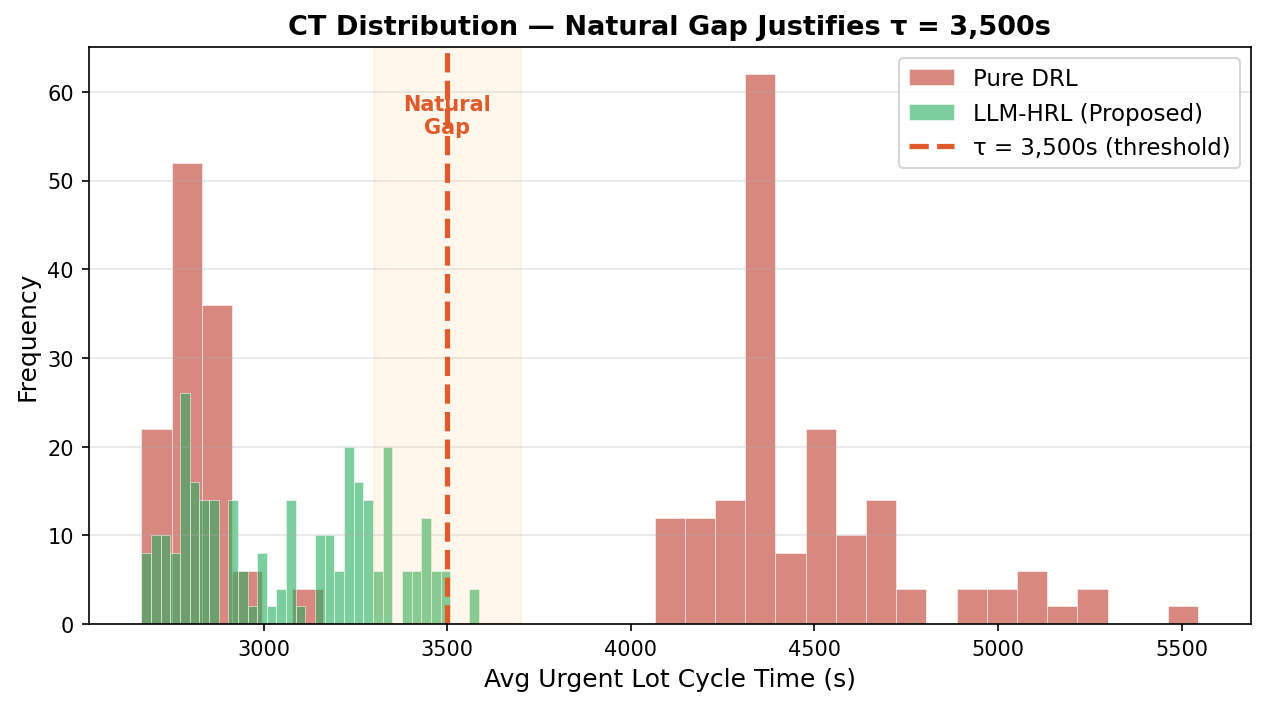
\includegraphics[width=0.98\linewidth]{ct_distribution_tau_justify}
  \caption{Empirical CT distribution across all evaluation episodes
  ($N=5$ seeds, 20 urgent lots). Pure DRL produces a bimodal distribution
  with a cluster of successes near 2{,}800\,s and a cluster of failures
  above 4{,}300\,s. LLM-HRL concentrates entirely in the success cluster.
  The failure threshold $\tau=3{,}500$\,s (dashed) falls in the natural
  gap between the two modes, confirming it is not an artifact of
  threshold selection.}
  \label{fig:ctdist}
\end{figure}

\subsection{Conditions}
We compare two conditions that share an \emph{identical reward function} and
differ only in governance:
(i) \textbf{Pure DRL}: the Rainbow DQN agent with no L1/L2 layers; and
(ii) \textbf{LLM-HRL (proposed)}: the full three-layer framework. Holding the
reward fixed isolates the effect of governance and rules out confounds from
reward shaping.

\subsection{Reliability protocol}
A central methodological point (validated in Section~\ref{sec:nondeterminism}) is
that the digital twin is internally nondeterministic, so a single random seed
does not reproduce an outcome. The RL community has documented that single-run
comparisons are unreliable \parencite{henderson2018} and advocated distributional
reporting with uncertainty quantification \parencite{agarwal2021}. Following this
best practice, we run each condition for 5 independent seeds and report
\emph{failure rates} and variance, not single-run means. Because the digital
twin is internally nondeterministic (Section~\ref{sec:nondeterminism}), even
a fixed seed does not guarantee reproducibility; multiple independent seeds
are therefore necessary to obtain a distribution of outcomes. Each run
executes 100 episodes in total; Figure~\ref{fig:convergence} shows that
both seeds' reward curves stabilize well before episode 70, so the final 30
episodes (71--100) capture settled behavior. Evaluation metrics are collected
over this window, during which LLM-generated rules are frozen and the agent
acts greedily.

\begin{figure}[h]
    \centering
    
\includegraphics[width=0.98\linewidth]{fig_convergence}
    \caption{Two Pure-DRL runs (seed 42 and seed 123, 20 urgent lots, 100 episodes).
    Both curves stabilize well before the episode-70 boundary (dotted line),
    confirming that 100 episodes and a 30-episode evaluation window are
    sufficient to capture settled behavior. The eventual gap in evaluation
    CT---one run failing ($>$3{,}500\,s), the other passing---motivates the
    nondeterminism analysis in Section~\ref{sec:nondeterminism}.}
    \label{fig:convergence}
\end{figure}

\subsection{Agent configuration}
The tactical agent uses Rainbow DQN with hidden layers [1024, 512, 256], learning
rate $3\times10^{-4}$, discount $\gamma=0.98$, replay capacity 100k, multi-step
$n=3$, and target updates every 300 steps. Checkpoints are saved every 10
episodes for post-hoc analysis. All hyperparameters follow standard Rainbow DQN defaults \parencite{hessel2018} and are held fixed across
conditions.

% ============================ 5. RESULTS ============================
\section{Results}
\label{sec:results}


\subsection{Digital-twin nondeterminism}
\label{sec:nondeterminism}
\begin{figure}[thb]
    \centering
    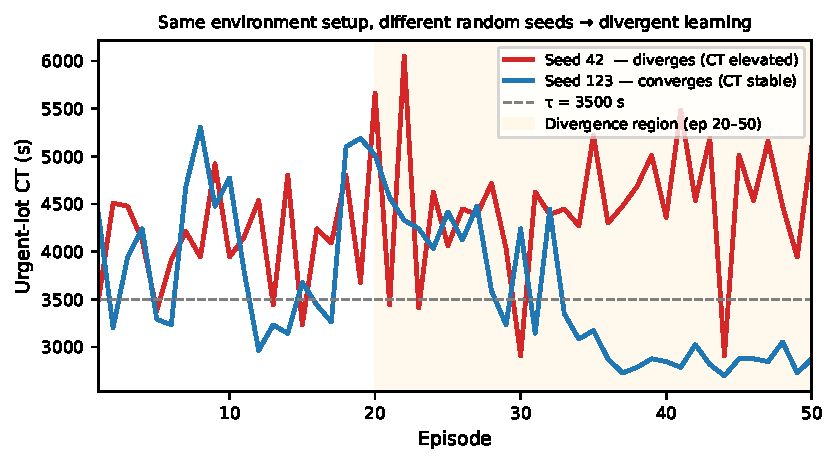
\includegraphics[width=0.98\linewidth]{fig_nondeterminism}
    \caption{Two Pure-DRL runs with \emph{identical} random seed and setup
    (20 urgent lots, 50 episodes). Both runs start from nearly the same CT
    trajectory but diverge around episode 20--25 as stochastic simulator-level
    timing differences---invisible to the Python RNG---compound through the
    learning process. Run~A converges to a passing policy
    (eval CT~2{,}274\,s) while Run~B settles into a failing one
    (eval CT~3{,}706\,s $> \tau$). The same nominal seed can therefore yield
    opposite outcomes, establishing that nondeterminism is intrinsic to the
    digital twin, not an artifact of seeding.}
    \label{fig:nondeterm}
\end{figure}

We establish that the digital twin's nondeterminism originates inside the
simulator, not in the Python RNG. With the Python-level random number
generators \emph{seeded identically}, two runs share near-identical
trajectories for the first $\sim$20 episodes but then diverge
(Figure~\ref{fig:nondeterm}): small, simulator-level timing differences
invisible to the Python RNG are amplified through the learning process,
causing the runs to settle into qualitatively different policies---one
converging to a passing cycle time (2{,}274\,s), the other remaining stuck
above the failure threshold (3{,}706\,s). The fault our governance layer
must tolerate is therefore intrinsic to the digital twin's stochastic
dynamics, not an artifact of implementation.

\subsection{Reliability: failure rate and variance}
\begin{table}[thb]
\centering
\setlength{\tabcolsep}{4pt}
\caption{Reliability results (20 urgent lots, $N=5$ seeds).}
\label{tab:reliability}
\begin{tabularx}{\columnwidth}{@{}Xcccc@{}}
\toprule
\textbf{Condition} & \textbf{Fail} & \textbf{CT mean} & \textbf{CT std} & \textbf{Worst} \\
\midrule
Pure DRL        & 60\% & 3{,}819\,s & 914\,s & 4{,}554\,s \\
LLM-HRL (ours)  & \textbf{0\%} & \textbf{3{,}071\,s} & \textbf{248\,s} & \textbf{3{,}309\,s} \\
\bottomrule
\multicolumn{5}{@{}l@{}}{\footnotesize $p{=}0.010$ binomial; $\Delta$CT $-19.6\%$; var.\ red.\ $73\%$}\\
\end{tabularx}
\end{table}

\begin{figure}[thb]
    \centering
    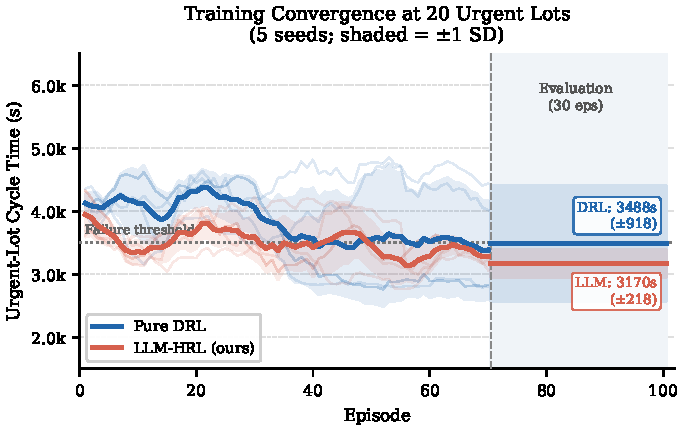
\includegraphics[width=0.98\linewidth]{fig_mechanism}
    \caption{Training convergence at 20 urgent lots (5 seeds; shaded band = $\pm$1\,SD).
    Both conditions stabilize before episode 70, confirming that the final
    30-episode evaluation window captures settled behavior.
    Pure DRL mean stays elevated and variable (eval CT 3{,}488\,s\,$\pm$918\,s),
    while LLM-HRL converges steadily to a low, stable cycle time
    (eval CT 3{,}170\,s\,$\pm$218\,s) with no failures across all seeds.
    The LLM intervenes on fewer than 2\% of evaluation steps, indicating that
    the value of governance lies in shaping the learned policy during training,
    not in runtime filtering.}
    \label{fig:mechanism}
\end{figure}

Table~\ref{tab:reliability} reports the central result for the primary
scenario (20 urgent lots). \textbf{Pure DRL failed catastrophically in 60\% of
runs ($\hat{\rho}_{\mathrm{DRL}} = 3/5$), whereas LLM-HRL failed in none
($\hat{\rho}_{\mathrm{LLM}} = 0/5$), giving $\Delta\rho = 0.60$.}
Under the one-sided null $H_0: \rho_{\mathrm{LLM}} \geq 0.60$ (LLM no better
than Pure DRL), the probability of $k=0$ failures in $N=5$ governed runs is
$p = \Pr(X \le 0 \mid X \sim \mathrm{Bin}(5,\,0.60))$, giving
\begin{equation}
  p = (1-0.60)^5 \approx 0.010,
  \label{eq:binomial}
\end{equation}
confirming that the failure-rate reduction is statistically significant at the
5\% level. The mean CT improved by 19.6\% (3{,}819\,s to
3{,}071\,s), and cycle-time variance fell by 73\% (std 914\,s to 248\,s),
reflecting the removal of the high-CT tail. Production attainment was
statistically unchanged across conditions ($p>0.05$), confirming that governance
removes the failure tail \emph{without} sacrificing throughput.

Per-seed detail (Figure~\ref{fig:perseed}) illustrates the nature of the
improvement. On the two seeds where Pure DRL succeeds (e.g.\ seed 123,
$\approx$2{,}820\,s), the governed agent matches it closely, confirming that
governance does not harm an already-converging run. On the three seeds where
Pure DRL fails (seeds 42, 2024, 7; CT $>4{,}400$\,s), the governed agent
attains CT in the 2{,}800--3{,}300\,s range, above the best DRL run but
far below the failure threshold. Governance is not a performance optimizer; it
is a failure preventer.

\begin{figure}[thb]
    \centering
    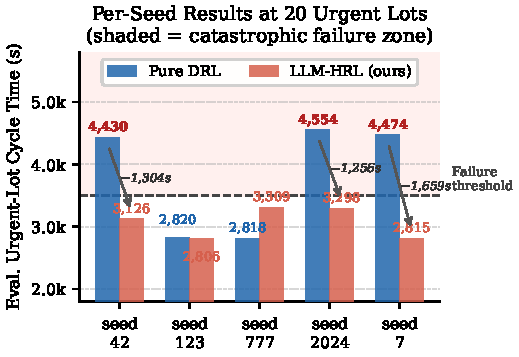
\includegraphics[width=0.98\linewidth]{fig_perseed}
    \caption{Per-seed evaluation CT at the primary scenario (20 urgent lots).
    Red shading marks the catastrophic-failure zone (CT $>$ 3{,}500\,s). Pure DRL
    fails on three seeds (42, 2024, 7) while LLM-HRL remains below the threshold
    on all five; arrows show the cycle-time reduction on failed DRL seeds.
    }
    \label{fig:perseed}
\end{figure}

\subsection{Production attainment under governance}
A necessary condition for the governed agent to be practically deployable is that
it does not sacrifice production throughput in pursuit of urgent-lot performance.
Table~\ref{tab:tmr} confirms this: Target Meet Rate (TMR) is statistically
indistinguishable between Pure DRL and LLM-HRL ($p > 0.05$, two-sample $t$-test).
Governance improves reliability without trading away throughput.

\begin{table}[thb]
\centering
\caption{Target Meet Rate (\%) by condition ($N=5$ seeds, 20 urgent lots,
mean\,$\pm$\,SD). No statistically significant difference ($p>0.05$).}
\label{tab:tmr}
\setlength{\tabcolsep}{4pt}
\begin{tabularx}{\columnwidth}{@{}XX@{}}
\hline
\centering\textbf{Pure DRL} & \centering\arraybackslash\textbf{LLM-HRL} \\ \hline
\centering $87.2 \pm 2.5$ & \centering\arraybackslash $86.1 \pm 2.7$ \\ \hline
\end{tabularx}
\end{table}

\subsection{How sparse governance shapes the policy}
A striking property is that the LLM intervenes on only a few percent of steps,
and during evaluation the frozen rules fire almost never, yet the governed agent
still attains a low, stable cycle time. This indicates that the value of
governance lies in \emph{when}, not \emph{how often}, it intervenes: a handful of
well-timed maskings during training (when an urgent lot is present and the urgent-lot action
should be taken) are sufficient to teach the agent to issue urgent priority,
a behavior Pure DRL acquires only by luck. The low masking rate at evaluation
($<$2\% of steps) confirms that governance's value lies in shaping the learned
policy during training rather than filtering at runtime---consistent with the
observation that LLM-HRL's CT distribution is tighter even when rules rarely
fire (Figure~\ref{fig:mechanism}).

\subsection{Ablation: value of adaptive LLM governance}
\label{sec:ablation}

To isolate the contribution of the LLM's \emph{adaptive} rule generation from
the mere presence of action constraints, we introduce a third condition:
\textbf{Rule-Based} --- a governance agent that applies the same L1 enforcement
mechanism as LLM-HRL but with a fixed, hand-crafted rule set derived from
domain knowledge, with no episodic LLM revision.
The rule set forbids non-urgent dispatching actions whenever
\texttt{urgent\_lot\_count\,$>$\,2}, mirroring the dominant pattern
the LLM discovers autonomously.
Note that this condition retains the same DRL agent (L0) and the same
rule-enforcement structure (L1) as LLM-HRL; only the L2 layer is replaced
by deterministic if-else logic. It is therefore distinct from the traditional
static dispatching rules evaluated in prior work~\parencite{lee2025}, which replace
the DRL agent entirely.
This ablation tests whether the LLM's episodic adaptation adds value beyond
simply having any rule-based constraint.

\begin{table}[thb]
\centering
\footnotesize
\caption{Ablation results (20 urgent lots, $N=5$ seeds).
Rule-Based applies a fixed domain rule without LLM adaptation;
LLM-HRL applies episodically revised LLM rules.}
\label{tab:ablation}
\setlength{\tabcolsep}{4pt}
\begin{tabularx}{\columnwidth}{@{}Xcccc@{}}
\toprule
\textbf{Condition} & \textbf{Fail} & \textbf{CT mean} & \textbf{CT std} & \textbf{Worst} \\
\midrule
Pure DRL        & 60\%          & 3{,}819\,s & 914\,s  & 4{,}554\,s \\
Rule-Based      & 60\%          & 3{,}347\,s & 543\,s  & 8{,}567\,s \\
LLM-HRL (ours)  & \textbf{0\%}  & \textbf{3{,}071\,s} & \textbf{248\,s} & \textbf{3{,}309\,s} \\
\bottomrule
\end{tabularx}
\end{table}

Rule-Based matches Pure DRL's 60\% failure rate while exhibiting a substantially
worse worst-case outcome (8{,}567\,s vs.\ 4{,}554\,s), confirming that
fixed action constraints alone do not confer reliability.
The LLM's \emph{adaptive, KPI-driven} revision is the operative mechanism.

% ============================ 6. DEPLOYMENT LESSONS ============================
\section{Deployment lessons: local-LLM rule generation}
\label{sec:lessons}

Operating a 7B local model as a control-rule generator surfaced systematic,
reproducible error patterns that any practitioner deploying LLM-in-the-loop
control should anticipate.

\subsection{Rule format, error taxonomy, and mitigation}
Each rule is a JSON tuple \texttt{(metric, operator, threshold,
forbidden\_actions, rationale)}; the rationale string provides a
human-readable audit trail absent from end-to-end DRL policies.
A representative well-formed rule reads:
\begin{quote}
\footnotesize\ttfamily
\{"metric": "urgent\_lot\_count",\\
\phantom{\{}"op": "{>}", "threshold": 2,\\
\phantom{\{}"forbidden": [0, 1, \ldots, 8],\\
\phantom{\{}"rationale": "prioritize urgent lots"\}
\end{quote}

Of 608 rules generated across our experiments,
14.5\% contained at least one defect, falling into three classes
(percentages sum to more than 14.5\% because a rule may exhibit multiple defects).

\noindent\textbf{(1) Scale confusion (9.0\%).} The LLM frequently copied an
\emph{episode-cumulative} KPI value (e.g.\ a count in the hundreds) into a
threshold that L1 evaluates against a \emph{per-step snapshot} (a count in the
low tens). Such rules can never fire and silently disable governance.

\noindent\textbf{(2) Inverted logic (6.7\%).} The model sometimes used
``$\leq$''/``$<$'' operators on metrics for which higher means worse, causing the
rule to trigger in \emph{normal} conditions and mask actions almost constantly.

\noindent\textbf{(3) Critical-action suppression (2.6\%).} The model
occasionally forbade the urgent-lot action itself, e.g.\ in
response to a production-shortage metric, directly undermining the behavior we
intend to encourage.

All three classes are detectable by lightweight structural checks: scale confusion
is caught by comparing the threshold against known per-step KPI ranges; inverted
logic by verifying that the operator direction matches the metric's polarity; and
critical-action suppression by explicitly rejecting any rule whose forbidden set
includes the urgent-lot action. A \emph{code-level sanitizer} applies these checks
deterministically at rule-ingestion time, correcting every defect before it
reaches L1 and yielding rules that are safe by construction. The sanitizer is
the concrete ``fault-removal'' mechanism that makes an imperfect local LLM safe
to deploy in the control loop: the language model supplies strategic intent,
while lightweight code guarantees that intent is expressed in valid, safe rules.


% ============================ 7. DISCUSSION ============================
\section{Discussion}
\label{sec:discussion}

Our results invite a reframing of what LLM-over-DRL governance is \emph{for}. The
governed agent does not outperform a \emph{lucky} Pure-DRL run; both converge to a
similar cycle time. Its value is that it eliminates the \emph{unlucky} runs, the
catastrophic schedules that arise intermittently from digital-twin
nondeterminism. In a manufacturing context, where a single badly scheduled urgent
lot can cascade into quality-time violations and yield loss, removing the failure
tail is often worth more than a marginal improvement in the average.

This perspective aligns the contribution with dependability engineering
\parencite{avizienis2004} rather than with leaderboard-style performance optimization.
Applying the Laprie fault--error--failure taxonomy to our setting:
the \textbf{fault} is simulator-level nondeterminism that the scheduler cannot
observe or control; the \textbf{error} is a learned policy that under-prioritizes
urgent lots when the fault corrupts the reward signal during training; and the
\textbf{failure} is $\overline{\mathrm{CT}}_i > \tau = 3{,}500$\,s, the
service-level consequence that triggers yield and delivery penalties on the shop
floor. LLM governance is accordingly a \emph{fault-tolerance mechanism}: it does
not eliminate the fault but breaks the fault$\to$error$\to$failure chain by
steering the policy toward correct behavior during training --- much as redundancy
or graceful degradation does in classical fault-tolerant systems. We report
\emph{failure rates}, not single-run means, because the quantity we seek to
improve is a property of the outcome distribution.

The governance overhead is negligible: one LLM call per episode ($\approx$2--5\,s
on a mid-range GPU), a rule set of typically 2--4 rules, and an L1 evaluation
cost of microseconds per step. This makes the approach practical even for
near-real-time dispatch cycles.

The explanation for the Rule-Based result is instructive: a static rule that forbids production-dispatching
actions whenever urgent lots are present constrains the agent's exploration even
during episodes where no urgent conflict arises, persistently distorting the
reward signal in the same way that reward up-weighting does.
Pure DRL retains the freedom to occasionally discover a good policy by chance;
Rule-Based forecloses that path, with the result that its failure cases are
structurally worse (higher worst-case CT). The LLM sidesteps this entirely by
intervening \emph{selectively}---only when KPIs signal an active conflict---leaving
the reward signal and exploration undistorted during normal operation. The ablation
therefore clarifies the central claim: it is not the \emph{presence} of a
constraint that matters, but its \emph{contextual, adaptive} application.

\subsection{Implications for socio-technical deployment}
The three-layer architecture maps naturally onto organizational roles: L0 is the
automated dispatcher, L1 enforces procedural rules at machine speed, and L2 acts
as a \emph{shift supervisor} that reviews KPIs and revises guidelines once per
episode. Because each rule carries an explicit natural-language rationale, a structured
audit trail supports the traceability required for
certification in safety-critical manufacturing automation, a property that purely
data-driven schedulers cannot provide. From an explainable-AI perspective, the
natural-language rationale attached to each rule makes governance decisions
interpretable to process engineers without specialist ML knowledge: operators
can inspect \emph{why} an action was forbidden, judge whether the rule reflects
a genuine operational concern, and override or refine it before the next
episode. This closes a key gap in autonomous scheduling systems, where
black-box DRL policies offer no such accountability channel.

% ============================ 8. CONCLUSION ============================
\section{Conclusion}
We presented a three-layer, locally hosted LLM-governed HRL framework for
urgent-lot scheduling in a semiconductor-manufacturing digital twin built from
real factory data.
Under the intrinsic nondeterminism of the high-fidelity simulator,
Pure DRL fails catastrophically in 60\% of independent runs;
our LLM-governed agent failed in 0\% ($p=0.010$, one-sided binomial, $N=5$ seeds),
reducing cycle-time variance by 73\% with no loss of production attainment.
The CT distributions of the two conditions form clearly separated clusters
with a natural gap at the chosen failure threshold $\tau=3{,}500$\,s,
confirming that the result is not an artifact of threshold selection.
We further demonstrated that the governance effect arises from correcting the
DRL training trajectory rather than imposing runtime constraints: masking
activity falls below 2\% at evaluation time, yet the learned policy is
consistently dependable.
Finally, we characterized the rule-generation error patterns of a local 7B
model and described the sanitizer pipeline that eliminates residual errors
before enforcement.
We argue that LLM governance is best understood not as a performance optimizer
but as a \emph{fault-tolerance mechanism} for learned components in
socio-technical manufacturing systems, and that the combination of a
high-fidelity digital twin with episodic LLM oversight offers a practical
path toward deploying dependable reinforcement learning in real semiconductor fabs.

% ============================ LIMITATIONS ============================
\section{Limitations and Future Work}
\label{sec:limitations}

\textbf{Digital-twin fidelity vs.\ live deployment.}
The digital twin used in this study was constructed from real semiconductor
factory data and validated against observed production statistics, providing
a high-fidelity experimental substrate.
However, all experiments are conducted in simulation; actual deployment to a
live fab would require additional integration work, real-time communication
interfaces with shop-floor equipment, and formal safety qualification
(e.g., IEC~61508 SIL assessment of the governance layer).
Live deployment is planned as future work in collaboration with the source
facility, and we expect the governance framework to transfer directly given
that the digital twin already replicates the production dynamics it would govern.

\textbf{Scope of the digital twin.}
The model represents a single line with six sequential process stages.
Generalization across lines, products, and model families has not been evaluated;
applying the methodology to a different fab or product mix will require
re-calibrating the digital twin and re-locating the sparsity regime in which
governance is most valuable.

\textbf{LLM rule quality.}
The local 7B model produced a 14.5\% rule-error rate, which the sanitizer
pipeline reduced to zero residual errors at runtime.
Upgrading to a larger instruction model or fine-tuning on domain-specific
scheduling data is expected to reduce the raw error rate and may allow
simplification of the sanitizer.

\printbibliography

\end{document}
